\documentclass[../../../main.tex]{subfiles}
\begin{document}
Les arbres constituent des structures \textit{non linéaires}, c'est-à-dire que les éléments ne sont pas stockés les uns à la suite des autres séquentiellement. Il s'agit en fait d'un cas particulier des graphes\footnote{Ce qui ne signifie pas que ce soit plus facile. Comme c'est simple mais qu'il faut faire des trucs intéressants avec, alors des gens un peu cinglés décident de complexifier à mort histoire qu'on y comprenne plus rien. Simple plaisir d'informaticien.}, comme cela sera vu plus tard.

Basiquement un arbre \textit{réel} peut être vu comme un racine à laquelle sont accrochées des branches. À chaque branche on trouve des noeuds qui donnent de nouvelles branches. Au bout de chaque branche il y a ou non une feuille.

L'avantage d'une telle structure peut être intuité comme suit : en partant de la racine et avançant de branche en branche vers une feuille, on atteint la feuille sans avoir parcouru toutes les branches ni toutes les feuilles de l'arbre.

L'idée est de construire formellement une structure équivalente avec cette propriété extraordinaire qui permette de limiter grandement la complexité des opérations d'accès aux données.
\subsection{Généralités sur les arbres quelconques}
On appelle \textit{arité} d'un arbre le nombre maximum de branches que peut avoir un noeud dans l'arbre.

\subsubsection{Noeud et racine}
On observe que la racine d'un arbre est un noeud comme les autres. Il a simplement la propriété d'être le noeud premier, qui n'a pas de noeud \textit{parent}. Si la racine a une branche vers un noeud, on peut à l'inverse considérer ce noeud comme la racine d'un sous-arbre.

Ainsi, un arbre $T$ d'arité $n$ est la donnée d'un noeud racine $r$ et d'au plus $n$ sous-arbres $t_1, \dots, t_n$ chacun d'arité $n$. On peut avoir exactement $n$ sous-arbres à chaque fois si on complète par une \textit{absence d'arbre}, qu'on appelle l'\textit{arbre vide} $E$.
\subsubsection{Feuilles}
Une feuille peut être vue comme un noeud\dots qui n'a pas de branches. C'est-à-dire que tous les sous-arbres sont absents. On définit donc une feuille comme un noeud dont tous les sous-arbres sont $E$.

\textbf{Remarque :} avec cette définition, une feuille forme toujours un arbre.
\subsection{Principe}
On s'arrête ici aux abres binaires\footnote{Y a déjà assez à faire comme ça\dots}, c'est-à-dire d'arité 2.

\textbf{Remarque :} Comme pour les listes, on va différencier un noeud $n$ de l'arbre de son contenu enregistré $x_n$. Il sera ainsi possible de considérer des arbres binaires dont chaque noeud stockera toutes les informations que l'on veut puisqu'on peut choisir un ensemble arbitraire pour les $x_i$

\textbf{Exemple :} Ci-dessous, un arbre\footnote{Les informaticiens, ne sortant jamais de leur cave où ils restent le nez rivé sur leur écran, n'ont jamais vus ni vrai herbe, ni vrai arbre. Ça explique pourquoi leurs représentations d'arbres sont à l'envers\dots} binaire à 6 noeuds : $0, \dots, 5$. $0$ est la racine. Les arbres vides $E$ ne sont pas montrés pour alléger le schéma.
\begin{center}
	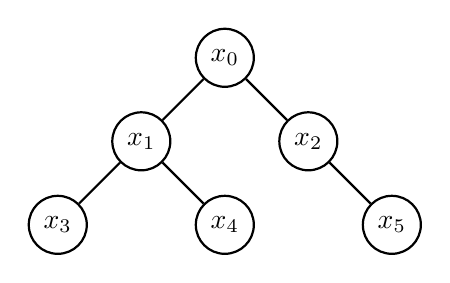
\begin{tikzpicture}[node distance={15mm}, thick, main/.style = {draw, circle}] 
	% Sommets :
	\node[main] (0) {$x_0$}; 
	\node[main] (1) [below left of=0] {$x_1$};
	\node[main] (2) [below right of=0] {$x_2$};
	\node[main] (3) [below left of=1] {$x_3$};
	\node[main] (4) [below right of=1] {$x_4$};
	\node[main] (5) [below right of=2] {$x_5$};
	% Arêtes
	\draw (0) -- (1);
	\draw (0) -- (2);
	\draw (1) -- (3);
	\draw (1) -- (4);
	\draw (2) -- (5);
	\end{tikzpicture} 
	\captionof{figure}{ Un arbre binaire\label{fig:abre_bin}}
\end{center}
\textbf{Détails :}
\begin{itemize}
	\item l'arbre de racine $3$ a $E$ comme sous-arbre à gauche comme à droite. On note cet arbre $a_3 = (E, x_3, E)$
	\item \textit{idem} pour l'arbre de racine $4$, on a $a_4 = (E, x_4, E)$
	\item \textit{idem} pour l'arbre de racine $5$, on a $a_5 = (E, x_5, E)$
	\item l'arbre de racine $1$ est donc $a_1 = (a_3, x_1, a_4)$
	\item l'arbre de racine $2$ est donc $a_2 = (E, x_2, a_5)$
	\item la racine de l'arbre total est $0$. L'arbre total est noté $A = (a_1, x_0, a_2)$
\end{itemize}
On peut définir de la même façon n'importe quel arbre par induction\footnote{Récurrence généralisée à n'importe quel type d'objet avec un ensemble de base défini par une règle $\mathcal{B}$ et une induction $\mathcal{I}$ sur l'ensemble} sur ses sous-arbres :
\definition{Arbres binaires} {
On appelle $E$ l'arbre vide. 

On note $A_{X}$ l'ensemble des arbres binaires définis sur un ensemble $X$. $A_{X}$ est définit par induction par les règles :
$$\left\{\begin{array}{cll}
	\mathcal{B} & : & E\in{A_{X}} \\
	\mathcal{I} & : & \forall{x\in{X}}, \forall{g, d\in{A_{X}}}, (g, x, d)\in{A_{X}}
\end{array}\right.$$

Pour tout $a = (l, x, r)\in{A_{X}\setminus{\{E\}}}$, $x$ est appelé la racine de $a$. $l$ et $r$ sont respectivement les enfants gauche et droit de $a$.
}
\textbf{Exemple :} On pose $X = \mathbb{N}$. On a $E$ un arbre (l'arbre vide), donc $(E, 5, E)$ est un arbre, donc $((E, 5, E), 2, E)$ est aussi un arbre, etc\dots
\definition{Hauteur d'un arbre} {
Soit $A_X$ un ensemble d'arbres binaires définies sur un ensemble $X$. La hauteur d'un arbre $a\in A_X$ est ``son nombre d'étages''. On définit alors la fonction hauteur $h : A_{X} \rightarrow{\mathbb{N}\cup\{-1\}}$ par induction selon les règles :
$$\left\{\begin{array}{cll}
	\mathcal{B} & : & h(E) = -1 \\
	\mathcal{I} & : & \forall{a = (g, x, d)\in{A_{X}}\setminus{\{E\}}}, h(a) = max(h(g), h(d)) + 1
\end{array}\right.$$
}
\textbf{Remarque :} On choisit une hauteur de $E$ négative pour que la hauteur soit le nombre d'étages de branches. Un arbre constitué d'une racine seule $(E, x, E)$ n'a pas d'étages. Sa hauteur est donc $0$. On utilisera la même notation pour les démonstrations sur les partitions d'ensembles finis en section \ref{sec:partitions}.

\textbf{Exemple :} sur la figure \ref{fig:abre_bin} :
\begin{itemize}
	\item $h((g, x_0, d)) = 2$
	\item $h((g, x_1, d)) = h((g, x_2, d)) = 1$
	\item $h((E, x_3, E)) = h((E, x_4, E)) = h((E, x_5, E)) = 0$
\end{itemize}
\subsection{Signature et implantation}
La définition d'un arbre montre que tout arbre peut être construit par composition d'autres arbres. On en déduit la signature :

\textit{ArbreBinaire\textless{}Element\textgreater} utilise \textit{Booleen}, \textit{Element}
\begin{itemize}
	\item $arbrevide()\rightarrow E$ renvoie la constante $E$ d'arbre vide.
	\item $creer(Element:x) \rightarrow ArbreBinaire$ renvoie l'arbre $(E, x, E)$
	\item $contenu(ArbreBinaire:T)\rightarrow Element$ où $T = (g, x, d)$ renvoie $x$. Indéfini si $T = E$
	\item $arbre\_droit(ArbreBinaire:T)\rightarrow ArbreBinaire$ où $T = (g, x, d)$ renvoie $d$. Indéfini si $T = E$
	\item $arbre\_gauche(ArbreBinaire:T)\rightarrow ArbreBinaire$ où $T = (g, x, d)$ renvoie $g$. Indéfini si $T = E$
	\item $construire(ArbreBinaire:g, Element:x, ArbreBinaire:d)\rightarrow ArbreBinaire$ renvoie l'arbre $(g, x, d)$
	\item $fixer\_contenu(ArbreBinaire:T, Element:x)\rightarrow ArbreBinaire$ où $T = (g, \dots, d)$ renvoie $(g, x, d)$
	\item $fixer\_droit(ArbreBinaire:T, ArbreBinaire:d)\rightarrow ArbreBinaire$ où $T = (g, x, \dots)$ renvoie $(g, x, d)$
	\item $fixer\_gauche(ArbreBinaire:T, ArbreBinaire:g)\rightarrow ArbreBinaire$ où $T = (\dots, x, d)$ renvoie $(g, x, d)$
	\item $chercher(ArbreBinaire:T, Element:x)\rightarrow Booleen$ teste si $x$ apparaît dans un des noeuds de l'arbre
\end{itemize}
En C, on peut, par exemple, utiliser des pointeurs d'arbres et poser par convention $E = \textsf{NULL}$ :
\begin{minted}[linenos=false]{c}
#include "element.h"

typedef struct TreeNode TreeNode; // Tree est un type pointeur vers struct Tree
typedef TreeNode Tree;
struct TreeNode {
	Tree* left;
	Tree* right;
	TreeNode nd;
	Element x;

	// Plus des métadonnées sur le noeud comme :
	Tree* parent; // connaître le parent permet de remonter l'arbre depuis une feuille
	int h; // hauteur de l'arbre dont le noeud est la racine (utile plus tard pour l'équilibrage)
};

Tree* tree_empty() {
	return NULL; // = E
}

Tree* tree_create(Element x) {
	Tree* t = (Tree*)malloc(sizeof(Tree));
	t->left = NULL; // = E
	t->right = NULL; // = E
	t->x = x;

	t->parent = NULL; // la racine n'a pas de parent
	t->h = 0;
	return t;
}

void tree_destroy(Tree* t) {
	if (t != NULL) {
		tree_destroy(t->left);
		tree_destroy(t->right);
		free(t);
	}
}
\end{minted}
Sans plus de propriétés, les arbres binaires ne sont pas plus utiles que cela.

\textbf{Arbres en peigne :} Les arbres binaires sont une généralisation des listes. En construisant un arbre avec seulement des enfants droits d'enfants droits d'enfants  droits, etc\dots on obtient un arbre filiforme dit ``en peigne'' $$(E, x_1, (E, x_2, \dots, (E, x_n, E)\dots))$$ dont on peut se convaincre aisément qu'il ne s'agit que d'une liste $[x_1, \dots, x_n]$. On cherche généralement à éviter ce cas de figure. En effet, l'accès à un élément devient fonction de $O(n)$ dans le pire des cas, où $n$ est le nombre d'éléments de l'``arbre''. Tout l'intérêt d'utiliser un arbre s'évapore. On présentera dans la suite une méthode d'équilibrage de l'arbre.
\subsection{Parcours d'arbres}
Les arbres sont des structures par nature récursives, puisque définies par induction. Le parcours des éléments d'un arbre peut donc naturellement être traité récursivement.

On distingue alors 3 types fondamentaux de parcours récursifs\footnote{On peut effectuer n'importe lequel des $n!$ parcours en soi. Mais ceux-là sont généralisables à tout arbre et peuvent posséder des propriétés utiles de temps en temps (ce qui n'est pas dit de parcours arbitraires).} : préfixe, suffixe et infixe. La différence est seulement l'ordre dans lequel chacun des noeuds est parcouru. Cet ordre peut avoir une importance si l'arbre possède des propriétés particulières (voir la sous-section \ref{sub:arbres_binaires_de_recherche})
\subsubsection{Parcours préfixe}
Dans un parcours préfixe, la racine de l'arbre est parcourue/traitée \textit{avant} de parcourir les sous-arbres gauche et droit :

\begin{algorithm}
\caption{Parcours récursif \textit{préfixe}\label{alg:arbre_parcours_prefixe}}
\SetKwFunction{parcoursrecursif}{\textsc{ParcoursPréfixe}}
\Indm\nonl\parcoursrecursif{$ArbreBinaire:A$, $Procedure:p$} \\
\Indp
\Switch {$A$} {
	\Case {$A = E$} { \tcp{Assure que l'algorithme termine puisque les sous-arbres finissent tous sur $E$}
	}
	\Case {$A = (g, x, d)$} {
		$p(x)$\;
		\parcoursrecursif{$g$, $p$}\;
		\parcoursrecursif{$d$, $p$}\;
	}
}
\end{algorithm}

\textbf{Construction de la liste de parcours :} Un arbre $A\neq E$ est la donnée d'un élément $x$ et de deux sous-arbres $g$ et $d$. Si on écrit le couple sous forme \textit{préfixe}, c'est-à-dire sous la forme $A = (x, g, d)$, en écrivant explicitement $A$ on obtient la liste $L$. Ainsi, en omettant les $E$ :
$$A = (0, (1, (3), (4)), (2, (5)))$$

Ainsi, pour l'arbre \ref{fig:abre_bin}, la liste des sommets parcourus est :
$$L = [0, 1, 3, 4, 2, 5]$$
\textbf{Remarque :} le parcours change si on écrit $A = (x, d, g)$ où $d$ est le sous-arbre droit de $A$ et $g$ le gauche.

\textbf{Interprétation :} on descend dans chaque sous-arbre en lisant un noeud dès qu'on le voit.
\subsubsection{Parcours suffixe}
Dans un parcours suffixe, la racine de l'arbre est parcourue/traitée \textit{après} avoir parcouru les sous-arbres gauche et droit :

\begin{algorithm}
\caption{Parcours récursif \textit{suffixe}\label{alg:arbre_parcours_suffixe}}
\SetKwFunction{parcoursrecursif}{\textsc{ParcoursSuffixe}}
\Indm\nonl\parcoursrecursif{$ArbreBinaire:A$, $Procedure:p$} \\
\Indp
\Switch {$A$} {
	\Case {$A = E$} {
		
	}
	\Case {$A = (g, x, d)$} {
		\parcoursrecursif{$g$, $p$}\;
		\parcoursrecursif{$d$, $p$}\;
		$p(x)$\;
	}
}
\end{algorithm}

\textbf{Construction de la liste de parcours :} Un arbre $A\neq E$ est la donnée d'un élément $x$ et de deux sous-arbres $g$ et $d$. Si on écrit le couple sous forme \textit{préfixe}, c'est-à-dire sous la forme $A = (g, d, x)$, en écrivant explicitement $A$ on obtient la liste $L$. Ainsi, en omettant les $E$ :
$$A = (((3), (4), 1), ((5), 2), 0)$$

Ainsi, pour l'arbre \ref{fig:abre_bin}, la liste des sommets parcourus est :
$$L = [3, 4, 1, 5, 2, 0]$$
\textbf{Remarque :} le parcours change si on écrit $A = (d, g, x)$ où $d$ est le sous-arbre droit de $A$ et $g$ le gauche.

\textbf{Interprétation :} on attend d'avoir vu tous les noeuds des sous-arbres avant de voir la racine.

\textbf{Exemple d'utilisation :} Par exemple, si une opération d'optimisation doit être effectuée sur un noeud qui dépend de l'opération effectuée sur chaque noeud des sous-arbres, le parcours suffixe permet de ``rassembler'' un maximum d'information pour avoir la meilleur opération d'optimisation.
\subsubsection{Parcours infixe}
Dans un parcours infixe, on traite d'abord le sous-arbre gauche, puis la racine, puis le sous-arbre droit. C'est le parcours infixe qui va être le plus utile dans la suite par sa propriété de conserver un ordre dans la liste de parcours de l'arbre.

\begin{algorithm}
\caption{Parcours récursif \textit{infixe}\label{alg:arbre_parcours_infixe}}
\SetKwFunction{parcoursrecursif}{\textsc{ParcoursInfixe}}
\Indm\nonl\parcoursrecursif{$ArbreBinaire:A$, $Procedure:p$} \\
\Indp
\Switch {$A$} {
	\Case {$A = E$} {
		
	}
	\Case {$A = (g, x, d)$} {
		\parcoursrecursif{$g$, $p$}\;
		$p(x)$\;
		\parcoursrecursif{$d$, $p$}\;
	}
}
\end{algorithm}

\textbf{Construction de la liste de parcours :} il suffit d'écrire un arbre $A\neq E$ comme habituellement sous la forme $A = (g, x, d)$ et de dérécursifier.
Ainsi, pour l'arbre \ref{fig:abre_bin}, la liste des noeuds parcourus est :
$$L = [3, 1, 4, 0, 2, 5]$$
\subsection{Arbres binaires de recherche}
\label{sub:arbres_binaires_de_recherche}
Les \underline{A}rbres \underline{B}inaires de \underline{R}echerche (ABR pour les intimes) forment l'application la plus commune des arbres binaires. Il s'agit d'un cas particulier dont les propriétés d'ordre sont très intéressantes. On peut par exemple utiliser les ABRs pour trier efficacement des tableaux d'éléments ou pour stocker efficacement des ensembles ordonnés.

L'ensemble $X$ des éléments d'un ABR doit être ordonné par une relation d'ordre partielle\footnote{Un ordre partiel est une contrainte suffisante, puisque le théorème de Szpilrajn affirme (démo rapide par lemme de Zorn) que toute relation d'ordre partielle peut être étendue en une relation d'ordre totale sur l'ensemble concerné.} $\leq_X$. On peut choisir par exemple $\mathbb{N}$, $\mathbb{Z}$ ou $\mathbb{R}$ munis de la relation d'ordre usuelle $\leq$.

\textbf{Notation :} pour définir formellement les arbres binaires de recherche, on note $elts:A\rightarrow \mathcal{P}(\mathbb{Z})$ la fonction qui à tout arbre associe l'ensemble des éléments de cet arbre.\newline
On définit formellement $elts$ par induction :
$$\left\{\begin{array}{cll}
	\mathcal{B} & : & elts(E) = \emptyset \\
	\mathcal{I} & : & \forall{a = (g, x, d)\in{A_{X}}\setminus{\{E\}}}, elts(a) = elts(g)\cup \{x\}\cup elts(d)
\end{array}\right.$$

\definition{Arbre binaire de recherche}{
	On note $A^{r}_\mathbb{X}$ l'ensemble des arbres binaires de recherche définis sur $A_{X}$ par induction par :
	$$\left\{\begin{array}{cll}
	\mathcal{B} & : & E\in A^r_X \\
	\mathcal{I} & : & \forall g, d\in A^r_X, \forall x\in X, \left[\forall{(n_{l}, n_{r})\in{elts(g)\times{elts(d)}}}, n_{l} \leq x \leq{n_{r}}\right] \Rightarrow (g, x, d)\in A^r_X
\end{array}\right.$$
Ce qu'on peut traduire en français par : les éléments du sous-arbre droit sont tous supérieurs ou égaux à la racine de l'arbre qui est elle-même supérieure ou égale à tous les éléments du sous-arbre gauche.
}
\textbf{Remarque :} Un arbre est construit comme des sous-arbres imbriqués. La propriété doit être vraie pour tout sous-arbre $(g, x, d)$ de l'arbre résultant de la racine primaire (c'est-à-dire celle sans parent)

\textbf{Exemple :} avec $X = \mathbb{N}$ muni de la relation d'ordre usuelle :
\begin{center}
	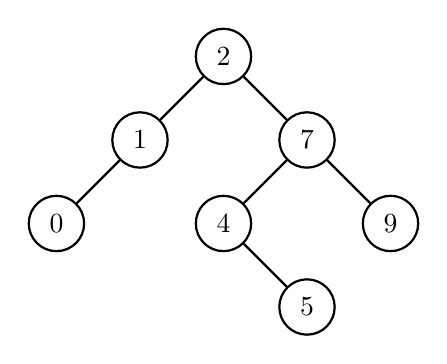
\begin{tikzpicture}[node distance={15mm}, thick, main/.style = {draw, circle, minimum size=2em}] 
	% Sommets :
	\node[main] (0) {2}; 
	\node[main] (1) [below left of=0] {$1$};
	\node[main] (2) [below right of=0] {$7$};
	\node[main] (3) [below left of=1] {$0$};
	\node[main] (4) [below right of=1] {$4$};
	\node[main] (5) [below right of=2] {$9$};
	\node[main] (6) [below right of=4] {$5$};
	% Arêtes
	\draw (0) -- (1);
	\draw (0) -- (2);
	\draw (1) -- (3);
	\draw (2) -- (4);
	\draw (2) -- (5);
	\draw (4) -- (6);
	\end{tikzpicture} 
	\captionof{figure}{Un ABR\label{fig:abr}}
\end{center}
\subsubsection{Signature}
La signature d'\textit{ABR} (pour \textit{ArbreBinaireDeRecherche}) est différente de celle d'un \textit{ArbreBinaire} puisqu'il faut supprimer toutes les routines de manipulation qui ne tiennent pas compte des propriétés d'ordre. Il faut en ajouter de nouvelles qui permettent de construire des \textit{ABR}.

\textit{ABR\textless{}Element\textgreater} utilise \textit{Booleen}, \textit{Element} :
\begin{itemize}
	\item $arbrevide()\rightarrow E$ renvoie la constante $E$ d'arbre vide.
	\item $creer(Element:x) \rightarrow ABR$ renvoie l'arbre $(E, x, E)$
	\item $contenu(ABR:T)\rightarrow Element$ où $T = (g, x, d)$ renvoie $x$. Indéfini si $T = E$
	\item $arbre\_droit(ABR:T)\rightarrow ABR$ où $T = (g, x, d)$ renvoie $d$. Indéfini si $T = E$
	\item $arbre\_gauche(ABR:T)\rightarrow ABR$ où $T = (g, x, d)$ renvoie $g$. Indéfini si $T = E$
	\item $chercher(ABR:T, Element:x)\rightarrow Boolen$ teste si $x$ apparaît dans un des noeuds de l'arbre
	\item $inserer(ABR:T, Element:x)\rightarrow ABR$ renvoie un arbre binaire de recherche contenant $elts(T)\cup\{x\}$
	\item $supprimer(ABR:T, Element:x)\rightarrow ABR$ renvoie un arbre binaire de recherche contenant $elts(T)\setminus\{x\}$
\end{itemize}

Ces routines sont les seules à pouvoir être utilisés en externe. Les routines elles-même peuvent en interne utiliser des routines de manipulation d'\textit{ArbreBinaire}. Pour rester rigoureux, on peut simplement considérer que les routines d'\textit{ArbreBinaire} restent définis \textit{si et seulement si} elles préservent la structure d'ABR.
\subsubsection{Recherche d'élément}
Si on veut trouver $x\in X$ dans un arbre $T = (g, y, d)$ et que $x \neq y$, alors selon la comparaison d'ordre entre $x$ et $y$ on sait dans quel sous-arbre $g$ ou $d$ chercher $x$ :
\begin{itemize}
	\item si $x < y$, $x\notin d$ par propriété d'ordre des ABRs, donc on cherche dans $g$
	\item si $x > y$, $x\notin g$ par propriété d'ordre des ABRs, donc on cherche dans $d$
\end{itemize}
\begin{algorithm}
\caption{Recherche d'un élément \label{alg:recherche_abr}}
\KwIn{$\textit{ABR\textless{}Element\textgreater}:T, Element:x$}
\While {$T\neq E \wedge contenu(T)\neq x$} {
	\eIf {$x \leq contenu(T)$} {
		$T\leftarrow arbre\_gauche(T)$\;
	} {
		$T\leftarrow arbre\_droit(T)$\;
	}
}
\Return $T\neq E$
\end{algorithm}
\textbf{Maximum et minimum :} pour trouver le maximum de l'arbre, il suffit d'aller toujours à droite, pour trouver le minimum de l'arbre, il suffit d'aller toujours à gauche.
\subsubsection{Insertion d'élément}
Pour insérer un élément, il suffit de chercher une place pour lui conserve la propriété d'arbre binaire de recherche. Or on sait comment chercher, il suffit d'effectuer des comparaisons successives avec les éléments rencontrés. Quand on descend dans l'arbre et qu'on rencontre un arbre vide, c'est là qu'il faut insérer l'élément.
\begin{algorithm}
\caption{Insertion d'un élément \label{alg:insertion_abr}}
\SetKwFunction{abrinserer}{\textsc{InsererElement}}
\Indm\nonl\abrinserer{$ABR:A$, $Element:x$} \\
\Indp
\Switch {$A$} {
	\Case {$A = E$} {
		\Return $(E, x, E)$
	}
	\Case {$A = (g, y, d)$} {
		\eIf {$x > y$} {
			$fixer\_droit(A, \abrinserer{d, x})$\;
		} {
			$fixer\_gauche(A, \abrinserer{g, x})$\;
		}
		\Return $A$
	}
}
\end{algorithm}
\textbf{Remarque :} on peut dérécursifier l'algorithme assez facilement ou l'écrire en récursif terminal. Dans les deux cas, on retire la nécessité de remonter la pile d'exécution, mais on ajoute plusieurs conditions supplémentaires.
\subsubsection{Suppression d'élément}
La suppression d'éléments dans un arbre est légèrement plus délicate pour s'assurer que l'arbre résultant est toujours un ABR. La recherche du noeud à supprimer est identique aux cas de recherche et d'insertion. Lorsqu'on trouve le noeud à supprimer $(g, x, d)$, si $d = E$ ou $g = E$, il suffit de remplacer le noeud par son seul sous-arbre différent de $E$. Dans le cas où chacun des deux sous-arbre est différent de $E$, il est très compliqué de supprimer le noeud tel quel. Par contre, on peut chercher à remplacer la valeur du noeud par celle d'un noeud du sous-arbre droit ou du sous-arbre gauche qui conserve l'ordre. Les deux seules valeurs possibles sont $max(elts(g))$ et $min(elts(d))$. On choisit donc arbitrairement entre les deux et on supprime le noeud correspondant après remplacement de $x$.

\begin{algorithm}
\caption{Suppression d'un élément \label{alg:suppression_abr}}
\SetKwFunction{parcoursrecursif}{\textsc{SupprimerMax}}
\Indm\nonl\parcoursrecursif{$ABR:A$, $Element:x$} \\
\Indp
\Case {$A = (g, y, E)$} {
	\Return $g$
}
\Case {$A = (g, y, d\neq E)$} {
	\Return \parcoursrecursif{d, x}
}
\SetKwFunction{abrsupprimer}{\textsc{SupprimerElement}}
\Indm\nonl\abrsupprimer{$ABR:A$, $Element:x$} \\
\Indp
\Switch {$A$} {
	\Case {$A = E$} {
		\Return $E$ \tcp*{Element pas présent dans l'arbre : rien à supprimer}
	}
	\Case {$A = (g, y, d)$} {
		\Case {$x > y$} {
			$fixer\_droit(A, \abrsupprimer(d, x))$\;
		}
		\Case {$x < y$} {
			$fixer\_gauche(A, \abrsupprimer(g, x))$\;
		}
		\Case {$x = y$} {
			\If {$d = E$} {
				\Return $g$
			}
			\If {$g = E$} {
				\Return $d$
			}
			$Element:m\leftarrow max(g)$\;
			$g\leftarrow \parcoursrecursif{g}$\;
			\Return $(g, m, d)$
		}
		\Return $A$
	}
}
\end{algorithm}
\subsubsection{Tri ABR}
\proposition{Ordre du parcours infixe} Le parcours infixe d'un arbre binaire de recherche $a\in A^r_X$ résulte en une liste triée selon la relation d'ordre sur $X$, avec une complexité temporelle fonction de $\Theta(n)$ où $n$ est le nombre d'éléments de $a$.

\textbf{Démonstration :} Le parcours visite les $n$ noeuds de l'arbre. La complexité est donc évidemment fonction de $\Theta(n)$. On montre le tri par induction, c'est-à-dire par \textit{initialisation} pour chaque élément défini par la règle de base $\mathcal{B}$ puis \textit{hérédité} selon la règle $\mathcal{I}$, où $\mathcal{B}$ et $\mathcal{I}$ sont les règles qui définissent l'ensemble des arbres binaires de recherches $A^r_X$.

\underline{Initialisation :} $E$ est sans éléments. Tout parcours de $E$ est vide donc trié.

\underline{Hérédité :} Soient $g, d\in A^r_X$ et $x\in X$. Supposons la proposition vraie pour $g$ et $d$. On suppose que pour tout $(a, b)\in elts(g)\times elts(d), a \leq x\leq b$. Par la règle d'induction $\mathcal{I}$, $(g, x, d)\in A^r_X$. Comme la liste $L(g)$ résultant du parcours infixe de $g$ et la liste $L(d)$ résultant du parcours infixe de $d$ sont triées, avec $x$ majorant de $elts(g)$ et minorant de $elts(d)$, alors la liste $L(g)::[x]::L(d)$ est triée. Il s'agit de la liste construite par l'algorithme \ref{alg:arbre_parcours_infixe} de parcours infixe sur $A^r_X$.

\textbf{Remarque :} Si on arrive à construire efficacement un arbre binaire de recherche à partir d'une liste non triée d'éléments, on peut trier efficacement cette liste par l'algorithme suivant :

\begin{algorithm}
\caption{Tri ABR\label{alg:arbre_tri_infixe}}
\KwIn{$\textit{Liste\textless{}Element\textgreater}:L$}
$\textit{ArbreBinaireRecherche\textless{}Element\textgreater}:abr \leftarrow construire(L)$\;
$L\leftarrow \textsc{ParcoursInfixe}(abr)$\;
\Return $L$\;
\end{algorithm}

Intuitivement, le plus simple est de partir d'un arbre vide et d'ajouter chacun des éléments de la liste en conservant la structure d'arbre binaire de recherche. Cependant, il faut faire attention à ce que l'arbre résultant soit bien ``équilibré'', notion à définir. 

\textbf{Arbres filiformes :} Comme on l'a observé précédemment, si l'arbre est \textit{filiforme}, de la forme $(E, e_1, (\dots, (E, e_n, E)\dots))$, on a juste une liste. L'ajout du $i^e$ élément a coûté le parcours de $i-1$ éléments. La complexité temporelle du tri est alors fonction de $O(n^2)$ par sommation des $i$ de $1$ à $n$. Il faut donc que l'arbre s'équilibre automatiquement au fur-et-à-mesure des insertions et des suppressions d'éléments.

Deux types d'arbres binaire de recherche auto-équilibrés sont communs :
\begin{itemize}
	\item les arbres \textit{AVL}\footnote{Du nom de leur inventeurs : M. Adelson-Velsky et M. Landis. C'est triste que M. Landis ait écopé d'une lettre de moins\dots}
	\item les arbres \textit{rouge-noir}\footnote{Notamment utilisés dans la bibliothèque standard C++ pour les ensembles et les dictionnaires ordonnés.}
\end{itemize}
Chacun est asymptotiquement équivalent en terme de classe de complexité temporelle. Les différences de performance se jouent principalement au niveau des constantes, qui diffèrent selon les opérations.
% De manière général, les constantes pour les arbres rouge-noir sont plus faibles, ce qui les rend plus rapides dans la pratique.\footnote{Ces arbres ne sont pas au programme de l'ISMIN, donc ils ne seront ajoutés que quand y aura le temps.}
\subsection{Arbres équilibrés}
\definition{Équilibre d'un arbre} {
	On définit l'équilibrage d'un arbre par la fonction :

	$$\begin{array}{lclcl}
	e & : & A_{X} & \rightarrow & \mathbb{Z}\\
	  &		& E & \mapsto & 0 \\ 
	  &		& (g, x, d) & \mapsto & h(d) - h(g)
\end{array}$$

	On dit alors qu'un arbre $T$ est \textit{équilibré} si et seulement si $|e(T)|\leq 1$. Il est dit \textit{déséquilibré} sinon.
}
\textbf{Interprétation :} Si la hauteur d'un sous-arbre d'un noeud est beaucoup plus grande que l'autre, c'est que les noeuds sont mal répartis entre les deux sous-arbres. On borne donc la différence de hauteur au minimum possible pour assurer la répartition des noeuds dans l'arbre.

\textbf{Remarque :} on a va s'intéresser dans la suite aux arbres qui sont à la fois des

\textbf{Exemples :} l'arbre de droite est déséquilibré car $e(2) = -2$. Tous les autres noeuds sont équilibrés.

\begin{minipage}{0.5\textwidth}
\begin{center}
	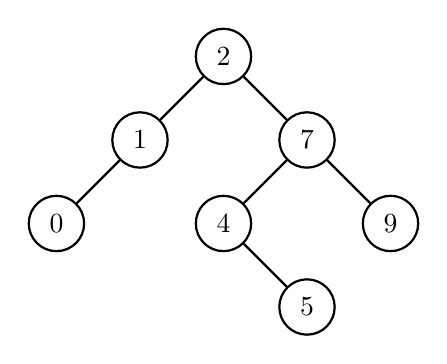
\begin{tikzpicture}[node distance={15mm}, thick, main/.style = {draw, circle, minimum size=2em}] 
	% Sommets :
	\node[main] (0) {2}; 
	\node[main] (1) [below left of=0] {$1$};
	\node[main] (2) [below right of=0] {$7$};
	\node[main] (3) [below left of=1] {$0$};
	\node[main] (4) [below right of=1] {$4$};
	\node[main] (5) [below right of=2] {$9$};
	\node[main] (6) [below right of=4] {$5$};
	% Arêtes
	\draw (0) -- (1);
	\draw (0) -- (2);
	\draw (1) -- (3);
	\draw (2) -- (4);
	\draw (2) -- (5);
	\draw (4) -- (6);
	\end{tikzpicture} 
	\captionof{figure}{ABR équilibré\label{fig:abr_equilibre}}
\end{center}
\end{minipage}
\begin{minipage}{0.5\textwidth}
\begin{center}
	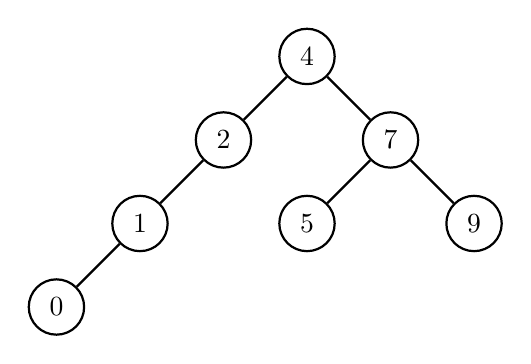
\begin{tikzpicture}[node distance={15mm}, thick, main/.style = {draw, circle, minimum size=2em}] 
	% Sommets :
	\node[main] (0) {4}; 
	\node[main] (1) [below left of=0] {2};
	\node[main] (2) [below right of=0] {$7$};
	\node[main] (6) [below left of=1] {$1$};
	\node[main] (3) [below left of=6] {$0$};
	\node[main] (4) [below left of=2] {$5$};
	\node[main] (5) [below right of=2] {$9$};
	
	% Arêtes
	\draw (0) -- (1);
	\draw (0) -- (2);
	\draw (1) -- (6);
	\draw (2) -- (4);
	\draw (2) -- (5);
	\draw (3) -- (6);
	\end{tikzpicture} 
	\captionof{figure}{ABR déséquilibré\label{fig:abr_desequilibre}}
\end{center}
\end{minipage}

\definition{Rotations gauche et droite} {
	Soit un arbre $T = ((A, x, B), y, C)$, avec $x,y \in X$ et $A, B, C\in A_X$.\newline

	On appelle \textit{rotation droite} l'opération :
	$$R_d(((A, x, B), y, C)) = (A, x, (B, y, C))$$
	On appelle \textit{rotation gauche} l'opération $R_g = R_d^{-1}$ inverse de $R_d$ :
	$$R_g((A, x, (B, y, C))) = ((A, x, B), y, C)$$
	Il est directement visible que le parcours infixe de l'arbre est invariant par chacune des rotations. En particulier, un arbre binaire de recherche qui subit des rotations gauche ou droite reste un arbre binaire de recherche
}
\textbf{Visuellement :} \begin{center}
		\includesvg[width=0.7\textwidth]{rotations}
		\captionof{figure}{Rotations (source : Wikipédia)}
	\end{center}
\proposition{Invariance de l'ordre par rotation} La propriété d'arbre binaire de recherche est invariante par les rotations gauche et droite.

\textbf{Démonstration :} voir la définition des rotations\footnote{Flemme de poser une induction aussi bateau.}

\proposition{Équilibrage par rotations} Soit $T = (g, x, d)$ un arbre déséquilibré dont les sous-arbres sont équilibrés.
\begin{itemize}
	\item si $e(T) < -1$
	\begin{itemize}
		\item si $e(g)\leq 0$, $R_d(T)$ améliore l'équilibrage de $T$
		\item si $e(g) = 1$, $R_d((R_g(g), x, d))$ améliore l'équilibrage de $T$
	\end{itemize}
	C'est-à-dire que ($e(T) < e(R_d((R_g(g), x, d))) \leq 1$ et $R_g(g)$ équilibré) ou $e(T) < R_d(T) \leq 1$
	\item si $e(T) > 1$
	\begin{itemize}
		\item si $e(d)\geq 0$, $R_g(T)$ améliore l'équilibrage de $T$
		\item si $e(d) = -1$, $R_g((g, x, R_d(d)))$ améliore l'équilibrage de $T$
	\end{itemize}
	C'est-à-dire que ($-1 \leq e(R_g((g, x R_d(d)))) < e(T)$ et $R_d(d)$ équilibré) ou $-1\leq e(R_g(T)) < e(T)$
\end{itemize}
\textbf{Démonstration} On ne traite que le cas $e(T) < -1$. Le second cas $e(T) > 1$ est symétrique.\newline
Soit $T = ((A, x, B), y, C)$ un arbre tel que :
\begin{itemize}
	\item $A$, $B$ et $C$ sont équilibrés.
	\item $(A, x, B)$ est équilibré, équivalent à $|h(A) - h(B)| \leq 1$
	\item $e(T) < -1$
\end{itemize}
\begin{itemize}
	\item Si $e(A, x, B) \leq 0$ :\newline
	Comme $e(T) < -1$, on a $h((A, x, B)) = max(h(A), h(B)) + 1\geq h(C) + 2$. \newline
D'où $max(h(A), h(B)) \geq h(C) + 1$. Dans tous les cas, on a $h(A)\geq h(C)$ et $h(B)\geq h(C)$ par l'équilibrage entre $A$ et $B$.
$$\begin{array}{lcl}
e(R_d(T)) - e(T) & = & max(h(C), h(B)) + 1 - h(A) - h(C) + 1 + max(h(A), h(B)) \\ 
& = & h(B) - h(A) + 1 + max(h(A), h(B)) + 1 - h(C) \\
& \geq & 3 + max(h(C), h(B)) - h(A) \\
& = & 3 + h(B) - h(A)\\ 
& > & 0
\end{array}$$
Donc $e(T) < e(R_d(T))$. Comme $h(B) - h(A) \leq 0$ :
$$\begin{array}{lcl}
e(R_d(T)) & = & max(h(B), h(C)) + 1 - h(A)\\
& = & h(B) + 1 - h(A) \\
& \leq & 1
\end{array}$$
	\item Si $e(A, x, B) = 1$, on a $B = (B_1, b, B_2)$. On a $h(B_1) = h(A)$ ou $h(B_1) = h(A) - 1$. \textit{idem} pour $h(B_2)$. Après rotation gauche de $(A, x, B)$, on a l'arbre $R_g(A, x, B) = ((A, x, B_1), b, B_2)$ qui n'est lui pas nécessairement équilibré. Par contre l'arbre $R_d(R_g(A, x, B), y, C)$ est lui équilibré et ses sous-arbres le sont. \newline
	En effet, $R_d(R_g(A, x, B), y, C) = ((A, x, B_1), b, (B_2, y, C))$. Comme $max(h(B_1), h(B_2)) = h(A)$ et $min(h(B_1), h(B_2)) \geq h(A)-1$, alors $(A, x, B_1)$ est équilibré de hauteur $h(A)$. On rappelle que $h(B) + 1\geq h(C) + 2$ donc $h(B_2)\geq h(C)$. Donc l'arbre $R_d(R_g(A, x, B), y, C)$ est équilibré à l'équilibrage de $(B_2, y, C)$ près. Si $h(B) = h(C) + 2$, l'arbre est équilibré. Si $h(B) > h(C) + 2$, $(B_2, y, C)$ est plus équilibré que l'arbre originel puisque $h(B_2) < h(B)$.
\end{itemize}
\textbf{Important :} on déduit de la démonstration que si $e(g, x, d) = -2$, soit $R_d(g, x, d)$ est équilibré, soit $R_d((R_g(g), x, d))$ est équilibré. \textit{idem} pour $e(g, x, d) = 2$. C'est cette propriété qui est utilisé pour l'implantation les arbres AVLs, notamment pour garantir l'équilibrage et par suite la complexité temporelle des opérations.

\textbf{Exemple :} La rotation droite du sous-arbre filiforme $(((E, 0, E), 1, E), 2, E)$ de la figure \ref{fig:abr_desequilibre} rééquilibre l'arbre :
\begin{center}
	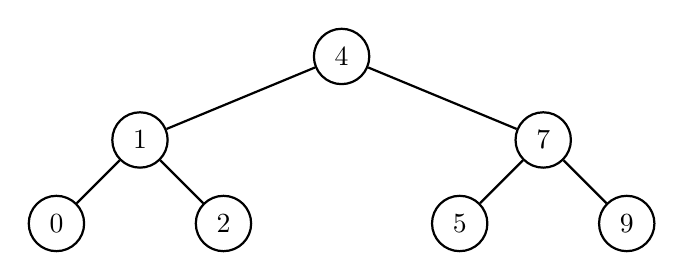
\begin{tikzpicture}[node distance={15mm}, thick, main/.style = {draw, circle, minimum size=2em}] 
	% Sommets :
	\node[main] (0) {4}; 
	\node[main] (1) [below left of=0, xshift=-15mm] {1};
	\node[main] (2) [below right of=0, xshift = 15mm] {$7$};
	\node[main] (6) [below right of=1] {$2$};
	\node[main] (3) [below left of=1] {$0$};
	\node[main] (4) [below left of=2] {$5$};
	\node[main] (5) [below right of=2] {$9$};
	
	% Arêtes
	\draw (0) -- (1);
	\draw (0) -- (2);
	\draw (1) -- (6);
	\draw (2) -- (4);
	\draw (2) -- (5);
	\draw (3) -- (1);
	\end{tikzpicture} 
	\captionof{figure}{ABR rééquilibré\label{fig:abr_reequilibre}}
\end{center}

\proposition{Hauteur d'un arbre strictement équilibré} La hauteur d'un arbre équilibré de $n$ éléments est fonction de $O(\log_2(n))$

\textbf{Démonstration :} On note alors $t(h)$ le nombre minimum d'élément d'un arbre équilibré $T$ de hauteur $h$. Pour maximiser la hauteur par rapport au nombre d'éléments, il faut que cet arbre soit déséquilibré d'un côté ou de l'autre, c'est-à-dire $e(T)\in\{-1, 1\}$. Pour maximiser la hauteur totale de $T$, on suppose que tout sous-arbre de $T$ est déséquilibré ainsi. On a donc :
$$\left\{\begin{array}{lcl}
t(0) & = & 1 \\
t(1) & = & 2 \\
t(h) & = & \underset{plus\ grand\ sous-arbre}{t(h - 1)} + \underset{plus\ petit\ sous-arbre}{t(h-2)} + \underset{racine}{1}
\end{array}\right.$$
On pose pour $h\in\mathbb{N}$, $F(h) = t(h) + 1$
$t(h + 2) = t(h+1) + t(h) + 1$ devient donc $F(h+2) = F(h+1) + F(h)$. L'équation caractéristique $r^2 - r - 1 = 0$ admet les deux racines $$r_1 = \phi = \dfrac{1 + \sqrt{5}}{2}\text{ et }r_2 = \dfrac{1 - \sqrt{5}}{2}$$
Il existe donc $\alpha,\beta\in\mathbb{R}$ tels que :
$$F(h) = \alpha r_1^h + \beta r_2^h$$
On a $F(0) = \alpha + \beta = 2$ et $F(1) = \alpha\dfrac{1 + \sqrt{5}}{2} + \beta\dfrac{1 - \sqrt{5}}{2} = 3$

D'où $\alpha = 1 + \dfrac{2}{\sqrt{5}}$ et $\beta = 1 - \dfrac{2}{\sqrt{5}}$.

Finalement,
$$t(h) = (1 + \frac{2}{\sqrt{5}})\phi^h + (1 - \frac{2}{\sqrt{5}})\left(\dfrac{1 - \sqrt{5}}{2}\right)^h - 1$$
Comme $\left|\dfrac{1 - \sqrt{5}}{2}\right| < 1$, il existe $C_1, C_2\in\mathbb{R}$ telle que $C_2\phi^h \leq t(h)\leq C_1\phi^h$

Si un arbre équilibré a $n$ élément, sa hauteur maximum $h(n)$ est fonction de $O(log_\phi(n) = O(log_2(n))$
\subsection{Arbres AVL}
\definition{Arbre AVL} {
	Un arbre AVL est un arbre binaire de recherche équilibré.\footnote{Selon le Cormen, référence du domaine. Wikipédia dit qu'un arbre AVL est juste un arbre équilibré. Mais alors, pourquoi Knuth dit ``balanced tree'' et pas ``AVL tree'' ? Parce-que l'article de Wikipédia a été écrit avec un manque de précision TERRIBLE, TERRIBLE je vous dis !}
}
Les opérations d'insertion, de suppression et de recherche sont donc de complexité temporelle fonction de $O(log_2(n))$, où $n\in\mathbb{N}$ est le nombre d'éléments de l'arbre.
\subsection{Exercices}
\exercise{Type abstrait d'arbre binaire} Implanter la signature d'\textit{ArbreBinaire} présenté dans le cours en C :
\begin{enumerate}
	\item d'abord avec les enregistrements proposés dans le cours
	\item ensuite avec un tableau qui contient tous les noeuds de l'arbre
\end{enumerate}

\exercise{Arbres binaire de recherche}{23} Implanter la signature d'\textit{ArbreBinaireDeRecherche} en C.\newline
\textit{\underline{Remarque :} identique à la structure d'un arbre binaire. La seule différence est dans le corps des routines, qui doit préserver la structure d'ordre, comme décrit dans le cours.}

\exercise{Arbres AVL}{30} \newline
Implanter des arbres AVLs en autoéquilibrant les ABRs de l'\refexercise{Arbres binaire de recherche} par des rotations durant les opérations d'insertion et de suppression. \newline
\textit{\underline{Notes :} il faut faire attention à ne pas oublier de modifier le pointeur vers le parent, où les prochaines rotations seront fausses. Utiliser un parcours récursif pour simplifier le code n'est pas absurde puisque la hauteur d'un arbre est logarithmique.}

\exercise{Arbres dimensionnels}{}

\exercise{Les tries}{}

\exercise{Codage de Huffman}{}

\exercise{Arbres auto-ajustés}{}
\end{document}
